% ============================================================
%  Thesis & Project Management System (TPMS)
%  Final Project Report — Minor Project (BE Computer Engineering)
%  Tribhuvan University, IOE, Pulchowk Campus
%
%  Authors : Prabesh BC, Shreeyut Thapa, Subesh Yadav
%  Batch   : 080BCT
%  Version : v2  (August 2026)
%  Template: Based on DOECE BE-Project LaTeX guidelines
% ============================================================

\documentclass[12pt]{report}

% ── Packages ────────────────────────────────────────────────
\usepackage[utf8]{inputenc}
\usepackage[T1]{fontenc}
\usepackage{xcolor}
\usepackage{natbib}
\usepackage[left=1.25in,right=1.0in,top=1.0in,bottom=1.0in]{geometry}
\usepackage{float}
\usepackage{graphicx}
\usepackage{rotating}
\usepackage{amsmath}
\usepackage{amssymb}
\usepackage{titlesec}
\usepackage{booktabs}
\usepackage{array}
\usepackage{longtable}
\usepackage{listings}
\usepackage{enumitem}
\usepackage{setspace}
\usepackage{microtype}
\usepackage{hyperref}
\usepackage{caption}

% ── Line spacing ─────────────────────────────────────────────
\linespread{1.3}

% ── Chapter / Section formatting ────────────────────────────
\titlespacing*{\chapter}{-15pt}{10pt}{15pt}
\titlespacing*{\section}{0pt}{8pt}{4pt}
\titlespacing*{\subsection}{0pt}{6pt}{3pt}
\titleformat{\chapter}[hang]
    {\normalfont\huge\bfseries}{\chaptertitlename\ \thechapter.}{1em}{}
\renewcommand{\chaptername}{}

% ── Graphics ─────────────────────────────────────────────────
\graphicspath{{Images/}}

% ── Hyperref setup ───────────────────────────────────────────
\hypersetup{
    colorlinks=true,
    linkcolor=black,
    citecolor=blue,
    urlcolor=blue,
    pdftitle={TPMS Final Report},
    pdfauthor={Prabesh BC, Shreeyut Thapa, Subesh Yadav},
    pdfsubject={Minor Project Report, BE Computer Engineering, IOE}
}

% ── Code listing style ───────────────────────────────────────
\definecolor{codegray}{rgb}{0.95,0.95,0.95}
\definecolor{codegreen}{rgb}{0,0.5,0}
\definecolor{codeblue}{rgb}{0,0,0.7}
\lstdefinestyle{tpmsstyle}{
    backgroundcolor=\color{codegray},
    commentstyle=\color{codegreen}\itshape,
    keywordstyle=\color{codeblue}\bfseries,
    basicstyle=\ttfamily\footnotesize,
    breaklines=true,
    frame=single,
    numbers=left,
    numberstyle=\tiny\color{gray},
    numbersep=5pt,
    tabsize=2,
    showstringspaces=false,
    captionpos=b
}
\lstset{style=tpmsstyle}

% ============================================================
\begin{document}

% ── Cover Page (manual titlepage) ────────────────────────────
\begin{titlepage}
\begin{center}

\includegraphics[scale=0.28]{logotu.jpg}\\[0.3cm]
\uppercase{\large
    Tribhuvan University\\
    Institute of Engineering\\
    Pulchowk Campus\\[0.5cm]
}
\vspace{0.4cm}
{\large A\\[0.2cm]Project Report\\[0.2cm]On}\\[0.4cm]
{\large\bfseries Thesis \& Project Management System (TPMS)}\\[0.8cm]
{\large \textbf{Submitted By:}\\[0.3cm]
 Prabesh BC \hspace{2mm}(PUL080BCT054)\\
 Shreeyut Thapa \hspace{2mm}(PUL080BCT080)\\
 Subesh Yadav \hspace{2mm}(PUL080BCT084)}\\[0.8cm]
{\large \textbf{Submitted To:}\\[0.2cm]
 Department of Electronics \& Computer Engineering}\\[1.0cm]
{\large August, 2026}
\end{center}
\end{titlepage}

\pagenumbering{roman}
\setcounter{page}{2}

% ── Page of Approval ─────────────────────────────────────────
\chapter*{Page of Approval}
\addcontentsline{toc}{chapter}{\numberline{}Page of Approval}
\vspace{1.5cm}
\begin{center}
\uppercase{
    Tribhuvan University\\
    Institute of Engineering\\
    Pulchowk Campus\\
    Department of Electronics and Computer Engineering
}
\end{center}
\vspace{0.5cm}

The undersigned certifies that they have read and recommended to the Institute of
Engineering for acceptance of a project report entitled \textbf{``Thesis \& Project
Management System (TPMS)''} submitted by \textbf{Prabesh BC (PUL080BCT054)},
\textbf{Shreeyut Thapa (PUL080BCT080)}, and \textbf{Subesh Yadav (PUL080BCT084)} in
partial fulfilment of the requirements for the Bachelor's degree in Computer Engineering.

\vspace{1.5cm}
\begin{minipage}{.5\textwidth}
    \raggedright
    ............................\\
    Supervisor\\
    \textbf{Er. Bishnu Tamang}\\
    Assistant Professor\\
    Department of Electronics and Computer Engineering,\\
    Pulchowk Campus, IOE, TU.
\end{minipage}%
\begin{minipage}{0.5\textwidth}
    \raggedleft
    ............................\\
    External Examiner\\
    \textbf{Dr. Kiran Mainali}\\
    Associate Professor\\
    Department of Electronics and Computer Engineering,\\
    Pulchowk Campus, IOE, TU.
\end{minipage}

\vspace{1.5cm}
\centerline{Date of approval: \underline{\hspace{5cm}}}

% ── Copyright ────────────────────────────────────────────────
\chapter*{Copyright}
\addcontentsline{toc}{chapter}{\numberline{}Copyright}
The authors have agreed that the Library, Department of Electronics and Computer
Engineering, Pulchowk Campus, and Institute of Engineering may make this report freely
available for inspection. Moreover, the authors have agreed that permission for
extensive copying of this project report for scholarly purposes may be granted by the
supervisor who supervised the work recorded herein or, in their absence, by the Head of
the Department wherein the project report was done. It is understood that recognition
will be given to the authors of this report and the Department of Electronics and
Computer Engineering, Pulchowk Campus, Institute of Engineering for any use of the
material of this project report. Copying, publication, or other use of this report for
financial gain without approval of the Department of Electronics and Computer
Engineering, Pulchowk Campus, Institute of Engineering, and the authors' written
permission is prohibited.

Request for permission to copy or to make any other use of the material in this report
in whole or in part should be addressed to:

\vspace{0.8cm}
Head\\
Department of Electronics and Computer Engineering\\
Pulchowk Campus, Institute of Engineering, TU\\
Lalitpur, Nepal.

% ── Acknowledgments ──────────────────────────────────────────
\chapter*{Acknowledgments}
\addcontentsline{toc}{chapter}{\numberline{}Acknowledgements}

We express our deepest gratitude to our project supervisor, \textbf{Er.\ Bishnu
Tamang}, Assistant Professor at the Department of Electronics and Computer Engineering,
Pulchowk Campus, for his invaluable guidance, continuous encouragement, and
constructive feedback throughout the development of this project.

We extend sincere thanks to \textbf{Prof.\ Dr.\ Sashidhar Ram Joshi}, Dean of the
Institute of Engineering, and the faculty members of the Department of Electronics and
Computer Engineering for providing the necessary infrastructure, laboratory facilities,
and a supportive academic environment.

We are grateful to the program coordinators and supervisors at Pulchowk Campus who
participated in our requirements analysis sessions and provided invaluable domain
expertise regarding evaluation workflows and institutional procedures.

Finally, we express heartfelt appreciation to our fellow classmates and family members
for their constant moral support and encouragement throughout this project.

% ── Abstract ─────────────────────────────────────────────────
\chapter*{Abstract}
\addcontentsline{toc}{chapter}{\numberline{}Abstract}

The management of undergraduate projects and postgraduate theses at Pulchowk Campus,
Institute of Engineering (IOE), has traditionally relied on fragmented manual
workflows, paper evaluation sheets, and uncoordinated communications. This paper-bound
paradigm results in supervision-tracking opacity, administrative bottlenecks during
evaluation periods, and error-prone mark aggregation.

To address these systemic inefficiencies, we present the \textbf{Thesis \& Project
Management System (TPMS)}, a comprehensive, secure, multi-tier web platform tailored
specifically to the academic governance structures of Pulchowk Campus. TPMS integrates
five distinct role-based access levels---Student, Supervisor, External Examiner,
Program Coordinator, and Maintainer---across six academic degree programmes (BCT, BEI,
MSNCS, MSICE, MSDSA, MSCSKE).

Built on a React~18 single-page application frontend and a Node.js Express REST API
backend connected to a PostgreSQL database via Prisma~ORM, TPMS encapsulates the
complete project lifecycle: group formation, bulk Excel student importing with anomaly
detection, supervisor assignment, document submission, criteria-based evaluation, and
headless \textbf{Puppeteer PDF rendering} of official, university-branded A4 evaluation
sheets with automatic mark-to-words conversion. Empirical validation demonstrates
100\% mark calculation accuracy and PDF generation under 1.2~seconds.

\vspace{0.5cm}
\noindent\textbf{Keywords:} \textit{Academic Management, Role-Based Access Control,
Headless PDF Rendering, Node.js, React, Prisma~ORM, PostgreSQL, Thesis Governance}

% ── Tables / Lists ───────────────────────────────────────────
\tableofcontents
\addcontentsline{toc}{chapter}{\numberline{}Contents}
\listoffigures
\addcontentsline{toc}{chapter}{\numberline{}List of Figures}
\listoftables
\addcontentsline{toc}{chapter}{\numberline{}List of Tables}

% ── List of Abbreviations ────────────────────────────────────
\chapter*{List of Abbreviations}
\addcontentsline{toc}{chapter}{\numberline{}List of Abbreviations}
\begin{tabular}{p{2.5cm} l}
\textbf{API}      & Application Programming Interface\\
\textbf{BCT}      & Bachelor in Computer Engineering\\
\textbf{BEI}      & Bachelor in Electronics, Communication \& Information Engineering\\
\textbf{CORS}     & Cross-Origin Resource Sharing\\
\textbf{DFD}      & Data Flow Diagram\\
\textbf{DOECE}    & Department of Electronics and Computer Engineering\\
\textbf{ER}       & Entity-Relationship\\
\textbf{HTML}     & HyperText Markup Language\\
\textbf{HTTP}     & Hypertext Transfer Protocol\\
\textbf{IOE}      & Institute of Engineering\\
\textbf{JWT}      & JSON Web Token\\
\textbf{MSDSA}    & MSc in Data Science and Analytics\\
\textbf{MSICE}    & MSc in Information and Communication Engineering\\
\textbf{MSNCS}    & MSc in Networked Computing Systems\\
\textbf{MSCSKE}   & MSc in Computer Science and Knowledge Engineering\\
\textbf{ORM}      & Object-Relational Mapping\\
\textbf{PDF}      & Portable Document Format\\
\textbf{RBAC}     & Role-Based Access Control\\
\textbf{REST}     & Representational State Transfer\\
\textbf{SPA}      & Single Page Application\\
\textbf{TPMS}     & Thesis \& Project Management System\\
\textbf{TU}       & Tribhuvan University\\
\textbf{UI}       & User Interface\\
\textbf{URL}      & Uniform Resource Locator\\
\end{tabular}

% ============================================================
%  CHAPTER 1: INTRODUCTION
% ============================================================
\chapter{Introduction}
\pagenumbering{arabic}

\section{Background}
Academic project work and thesis research represent the culmination of engineering
education at Pulchowk Campus, Institute of Engineering (IOE), Tribhuvan University.
Undergraduate students in Bachelor in Computer Engineering (BCT) and Bachelor in
Electronics, Communication \& Information Engineering (BEI) complete Minor Projects in
their third year and Major Projects in their fourth year. Concurrently, postgraduate
students across Master of Science programmes (MSNCS, MSICE, MSDSA, MSCSKE) conduct
thesis research spanning proposal defence, mid-term evaluation, and final defence.

Despite the high technical calibre of research produced, the administrative
orchestration of these activities has historically relied on physical paper evaluation
sheets, manual group-registration forms, notice-board announcements, and uncoordinated
email exchanges. Program coordinators face severe logistical overhead when managing
hundreds of enrolled students, mapping project groups to eligible supervisors,
distributing evaluation rubrics to external examiners, and compiling physical marks
into final grade sheets \citep{pressman2014software}.

Modern web engineering techniques combined with automated document compilation offer
an ideal solution for digitalising academic administration. The Thesis \& Project
Management System (TPMS) was conceived to replace paper-bound bottlenecks with a
unified, transparent, and resilient digital platform engineered specifically for
IOE DOECE standards.

\section{Problem Statement}
The legacy paper-based project and thesis management workflow at Pulchowk Campus
exhibits several critical operational drawbacks:

\begin{enumerate}[leftmargin=1.5cm]
    \item \textbf{High Administrative Burden:} Program coordinators manually track
          student groups, verify roll numbers, validate project titles, and match
          groups with available faculty supervisors using physical lists and spreadsheets.
    \item \textbf{Supervision \& Progress Opacity:} Students and department heads lack
          real-time visibility into supervisor assignment status, recommendation status,
          and evaluation schedules.
    \item \textbf{Error-Prone Evaluation Sheet Compilation:} Supervisors and external
          examiners manually record numerical marks, convert totals into words, and
          submit physical forms---frequently introducing transcription errors and delays.
    \item \textbf{Document Versioning Disarray:} Project proposals and thesis manuscripts
          are exchanged via scattered email attachments, resulting in loss of submission
          histories and inadequate version tracking.
    \item \textbf{Lack of Centralised Programme Visibility:} Coordinators for different
          degree programmes have no unified view of groups, theses, supervisor
          capacities, or evaluation completion status.
\end{enumerate}

\section{Objectives}
The primary objective of this project is to design, develop, test, and deploy a secure,
web-based Thesis \& Project Management System (TPMS) customised for Pulchowk Campus,
IOE. The specific sub-objectives are:

\begin{itemize}[leftmargin=1.5cm]
    \item To implement a granular 5-role security model (Student, Supervisor, External
          Examiner, Program Coordinator, Maintainer) with role-specific navigation and
          programme-scoped data access.
    \item To build an automated Excel batch import module capable of parsing class
          rosters, identifying data anomalies, and auto-provisioning student groups and
          supervisor assignments for both Bachelor projects and Master theses.
    \item To develop an interactive evaluation workbench with criteria-based mark entry,
          real-time total score calculation, and word-equivalent mark transformation.
    \item To integrate a server-side Puppeteer PDF rendering engine that generates
          official, university-formatted A4 evaluation sheets ready for signature and
          printing.
    \item To implement an announcement and academic-year management system that supports
          group formation workflows for Bachelor and Master degree programmes.
\end{itemize}

\section{Scope \& Limitations}
\textbf{Scope:} TPMS encompasses the academic administration of Minor/Major projects
for BCT and BEI programmes, as well as Master thesis and project workflows for MSNCS,
MSICE, MSDSA, and MSCSKE programmes within the DOECE department. It covers the full
evaluation lifecycle from group formation to PDF sheet generation.

\textbf{Limitations:}
\begin{itemize}[leftmargin=1.5cm]
    \item The current release focuses on departmental governance within DOECE and
          requires schema adaptations for campus-wide integration.
    \item Digital signature verification relies on physical printing rather than
          PKI hardware tokens.
    \item The system requires active network connectivity; offline mode is not yet
          supported.
\end{itemize}

% ============================================================
%  CHAPTER 2: LITERATURE REVIEW
% ============================================================
\chapter{Literature Review}

\section{Related Work}
Digital transformation in higher education administration has driven the adoption of
Learning Management Systems (LMS) such as Moodle and Canvas, alongside specialised
thesis repository systems like DSpace \citep{lewis2020retrieval}. However, commercial
LMS platforms primarily target course content delivery and gradebooks, failing to model
the complex academic project workflows required at IOE---such as multi-student group
formation, dual examiner assignment, 5-criteria rubric evaluation, and institutional
grade forwarding.

Prior work by \citet{giri2019transfer} highlighted the necessity of domain-specific
academic workflow automation in Nepali engineering institutions. Existing open-source
portals lack native PDF template compilation adhering to official IOE evaluation sheet
formats, forcing faculty to manually transcribe digital grades onto paper forms.

Commercial academic management tools are designed for Western institutional structures
and lack the role separation, multi-programme coordinator model, and headless PDF
generation capabilities required at Pulchowk Campus.

\section{Related Theory}

\subsection{Single-Page Application (SPA) Architecture}
Modern web applications leverage SPA patterns, where the browser loads a single HTML
shell and dynamically updates content via RESTful API calls without full page reloads.
React~18, utilising a virtual DOM and concurrent rendering, enables highly reactive UI
updates essential for multi-criteria evaluation workbenches and real-time mark
calculation \citep{fielding2000architectural}.

\subsection{RESTful API \& JWT Authentication}
Representational State Transfer (REST) provides a scalable client-server architectural
style. Authentication in stateless REST APIs is achieved via JSON Web Tokens (JWT). A
JWT consists of a Base64-encoded Header, Payload (containing user ID, role, and
programme scope), and a cryptographic Signature verified using HMAC-SHA256, allowing
each API request to be independently validated without server-side session storage.

\subsection{Object-Relational Mapping (ORM) with Prisma}
Database access in Node.js applications has evolved from raw SQL queries to type-safe
ORM layers. Prisma~5 uses a declarative schema specification (\texttt{schema.prisma})
to auto-generate JavaScript client bindings, enforcing foreign key integrity, schema
migrations, and relational eager loading. Prisma's \texttt{\$transaction()} API ensures
atomic multi-entity write operations during bulk imports.

\subsection{Server-Side Headless PDF Generation with Puppeteer}
Compiling dynamic HTML templates into print-ready A4 PDF documents requires headless
browser execution. Puppeteer controls headless Chromium via the Chrome DevTools
Protocol, executing pixel-perfect CSS Paged Media layout algorithms
(\texttt{@page \{ size: A4; margin: 15mm; \}}) to render university headers, logos, and
evaluation tables. This approach ensures the generated PDF is visually identical to a
browser-rendered page.

\subsection{Role-Based Access Control (RBAC)}
RBAC is a security model in which users are assigned one or more roles, and permissions
are defined at the role level. In TPMS, Express.js middleware intercepts every API
request, decodes the JWT, and checks whether the authenticated user's role is
authorised for the requested resource. Programme-scoped data filtering ensures that a
BCT coordinator sees only BCT data, even if they are also a supervisor for a Master
thesis.

% ============================================================
%  CHAPTER 3: METHODOLOGY
% ============================================================
\chapter{Methodology}

\section{Requirement Analysis \& Feasibility Study}
The methodology commenced with a comprehensive requirement-gathering phase involving
structured interviews with DOECE program coordinators, project supervisors, and
final-year BCT students at Pulchowk Campus. Observation sessions of the existing paper
evaluation process were conducted during the Spring~2026 evaluation period.

\textbf{Functional Requirements:}
\begin{itemize}[leftmargin=1.5cm]
    \item \textbf{FR1 (Authentication):} Secure login with role determination and
          bcryptjs password hashing.
    \item \textbf{FR2 (Group Formation):} Student-initiated group creation with
          invitation confirmation, roll number validation, and supervisor request.
    \item \textbf{FR3 (Bulk Import):} Excel file upload (\texttt{.xlsx}) by
          coordinators to auto-create thesis/group records and assign supervisors and
          examiners; supports both Bachelor projects and Master theses.
    \item \textbf{FR4 (Evaluation Workbench):} Rubric-based scoring
          (5 criteria $\times$ 20~marks $=$ 100~total) for Supervisor, Mid-Term
          External, and Final External evaluators.
    \item \textbf{FR5 (PDF Generation):} Automated creation of official TU/IOE
          evaluation sheets with marks-in-words conversion.
    \item \textbf{FR6 (Announcements):} Programme-specific announcements supporting
          group formation activation for Minor/Major/Master workflows.
\end{itemize}

\textbf{Non-Functional Requirements:}
\begin{itemize}[leftmargin=1.5cm]
    \item \textbf{NFR1 (Performance):} PDF generation under 1.5~seconds; page load
          under 2~seconds.
    \item \textbf{NFR2 (Security):} All endpoints protected by JWT; SQL injection
          prevented by ORM parameterisation.
    \item \textbf{NFR3 (Usability):} Role-specific dashboards; responsive design for
          laptop/desktop viewports.
    \item \textbf{NFR4 (Maintainability):} Modular Express route/controller structure;
          Prisma schema as single source of truth.
\end{itemize}

\textbf{Feasibility:} The technology stack (React~18, Node.js~20, Express,
PostgreSQL~16, Prisma~5, Puppeteer) consists entirely of open-source, enterprise-grade
frameworks with active community support and production readiness on Linux.

\section{Software Development Lifecycle (Agile Scrum)}
The system was developed following an Agile Scrum methodology over a 16-week timeline,
divided into four 4-week sprints:
\begin{itemize}[leftmargin=1.5cm]
    \item \textbf{Sprint 1 (W1--W4):} Database schema design, Prisma ORM migrations,
          JWT authentication system, user management endpoints, and programme/department
          seeding.
    \item \textbf{Sprint 2 (W5--W8):} Student group formation, group invitation system,
          proposal upload, coordinator dashboard, and announcement module.
    \item \textbf{Sprint 3 (W9--W12):} Evaluation workbench, Puppeteer PDF rendering
          engine, Excel bulk import with anomaly detection, and supervisor assignment.
    \item \textbf{Sprint 4 (W13--W16):} Master thesis workflow, RBAC hardening,
          integration testing, performance benchmarking, and documentation.
\end{itemize}

\section{Data Model Design}
The relational database was modelled in PostgreSQL via Prisma~ORM. Key entity
relationships are:
\begin{itemize}[leftmargin=1.5cm]
    \item \texttt{User} supports all five roles through a single entity with role enum
          and optional programme/department links.
    \item \texttt{ProjectGroup} (Bachelor) -- \texttt{GroupMember} (many students) --
          \texttt{EvaluationComponent} (evaluation stages).
    \item \texttt{Thesis} (Master) -- one \texttt{Student} -- one \texttt{Supervisor} --
          one \texttt{ExternalMidTerm} -- one \texttt{ExternalFinal} --
          \texttt{EvaluationComponent}.
    \item \texttt{EvaluationComponent} (1) $\rightarrow$ (0..1) \texttt{Evaluation}
          $\rightarrow$ JSON marks per criterion.
    \item \texttt{Announcement} (1) $\rightarrow$ ($N$) \texttt{ProjectGroup} or
          \texttt{Thesis} (type-scoped: MINOR / MAJOR / THESIS).
\end{itemize}

\section{Security \& RBAC Implementation}
Security is enforced at the API gateway level. Express middleware inspects incoming
\texttt{Authorization: Bearer <token>} headers, verifies the JWT signature, and checks
role authorisation before granting access:

\begin{lstlisting}[language=Java, caption={JWT RBAC Middleware (authMiddleware.js)}]
const authorize = (allowedRoles = []) => {
  return (req, res, next) => {
    const token = req.headers.authorization?.split(' ')[1];
    if (!token) return res.status(401).json({ error: 'Unauthorized' });
    try {
      const decoded = jwt.verify(token, process.env.JWT_SECRET);
      req.user = decoded;
      if (!allowedRoles.includes(req.user.role)) {
        return res.status(403).json({ error: 'Access Denied' });
      }
      next();
    } catch (err) {
      return res.status(401).json({ error: 'Invalid token' });
    }
  };
};
\end{lstlisting}

% ============================================================
%  CHAPTER 4: SYSTEM DESIGN
% ============================================================
\chapter{System Design}

\section{System Architecture}
TPMS utilises a 3-tier decoupled software architecture designed for high availability,
security, and clear separation of concerns, as illustrated in
Figure~\ref{fig:architecture}.

\begin{figure}[H]
    \centering
    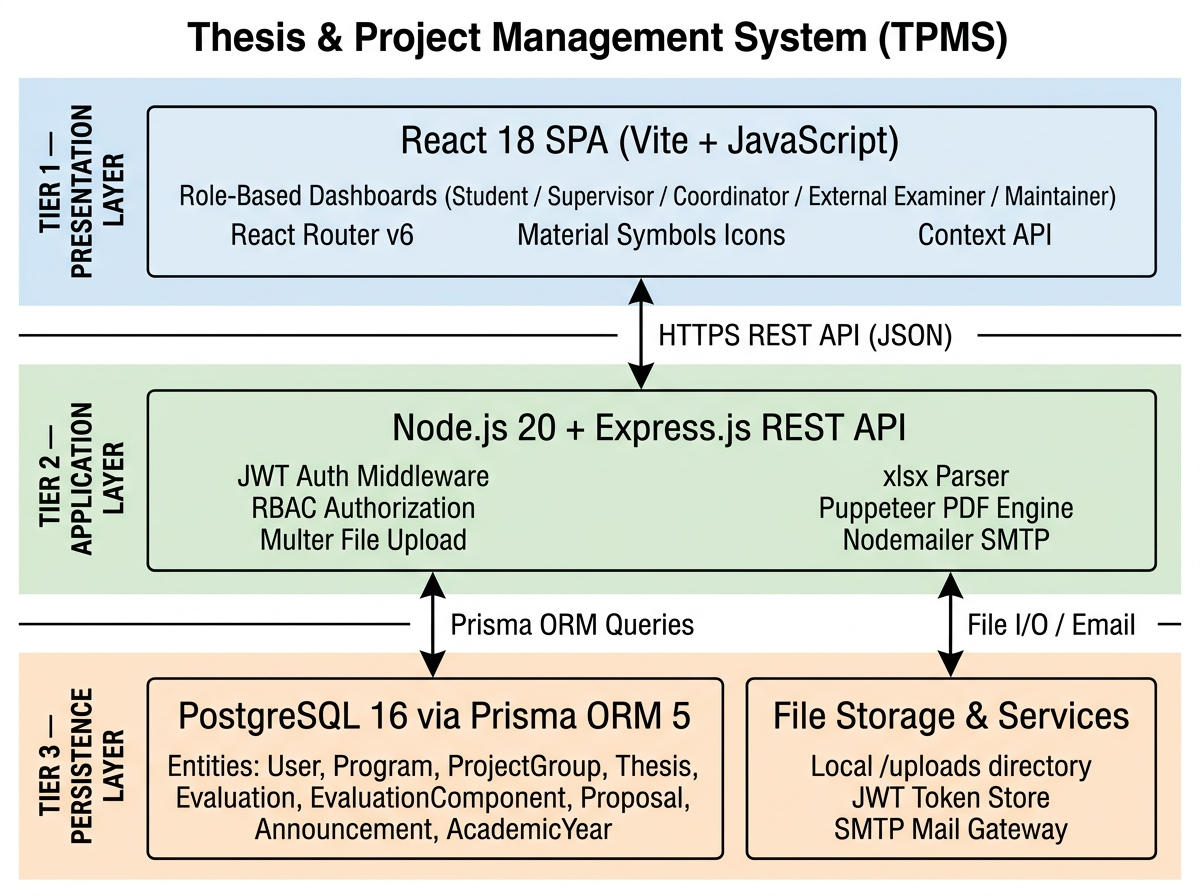
\includegraphics[width=0.97\textwidth]{fig_architecture.jpg}
    \caption{TPMS Three-Tier System Architecture}
    \label{fig:architecture}
\end{figure}

The architecture comprises three distinct tiers:
\begin{enumerate}[leftmargin=1.5cm]
    \item \textbf{Presentation Tier:} React~18 SPA built with Vite~5. Provides
          role-specific dashboards for all five user roles via React Router~v6. Global
          state managed via React Context API.
    \item \textbf{Application Tier:} Node.js~20 and Express.js REST API server.
          Handles JWT authentication, RBAC middleware, Multer file uploads, xlsx
          Excel parsing, Puppeteer PDF generation, and Nodemailer SMTP email.
    \item \textbf{Persistence Tier:} PostgreSQL~16 accessed via Prisma~ORM. Manages
          all persistent entities. Local \texttt{/uploads} directory stores uploaded
          proposal PDFs and Excel files.
\end{enumerate}

\section{Module Breakdown}
TPMS is organised into six core functional modules:

\begin{itemize}[leftmargin=1.5cm]
    \item \textbf{Auth Module:} User registration, bcryptjs password hashing, JWT
          issuance, and password reset via email token.
    \item \textbf{Group \& Thesis Module:} Bachelor project group formation with member
          invitations; Master thesis/project registration with programme, batch,
          cluster, and project-type assignment.
    \item \textbf{Import Module:} Excel parser, roll number verification, fuzzy name
          matching, anomaly detection preview, and atomic bulk transaction creation.
    \item \textbf{Evaluation Module:} Dynamic evaluation component loader, numerical
          criterion mark entry with live total calculation, marks-in-words conversion,
          and evaluation status tracking.
    \item \textbf{Print Engine:} Puppeteer HTML-to-PDF compilation for official
          TU/IOE evaluation sheets. Supports Supervisor, Mid-Term External, and Final
          External formats for both degree types.
    \item \textbf{Coordinator Module:} Supervisor assignment, external examiner
          assignment, academic year management, programme announcements, and result
          finalisation.
\end{itemize}

\section{Use Case Analysis}
The interactions between system actors and core use cases are depicted in
Figure~\ref{fig:usecase}.

\begin{figure}[H]
    \centering
    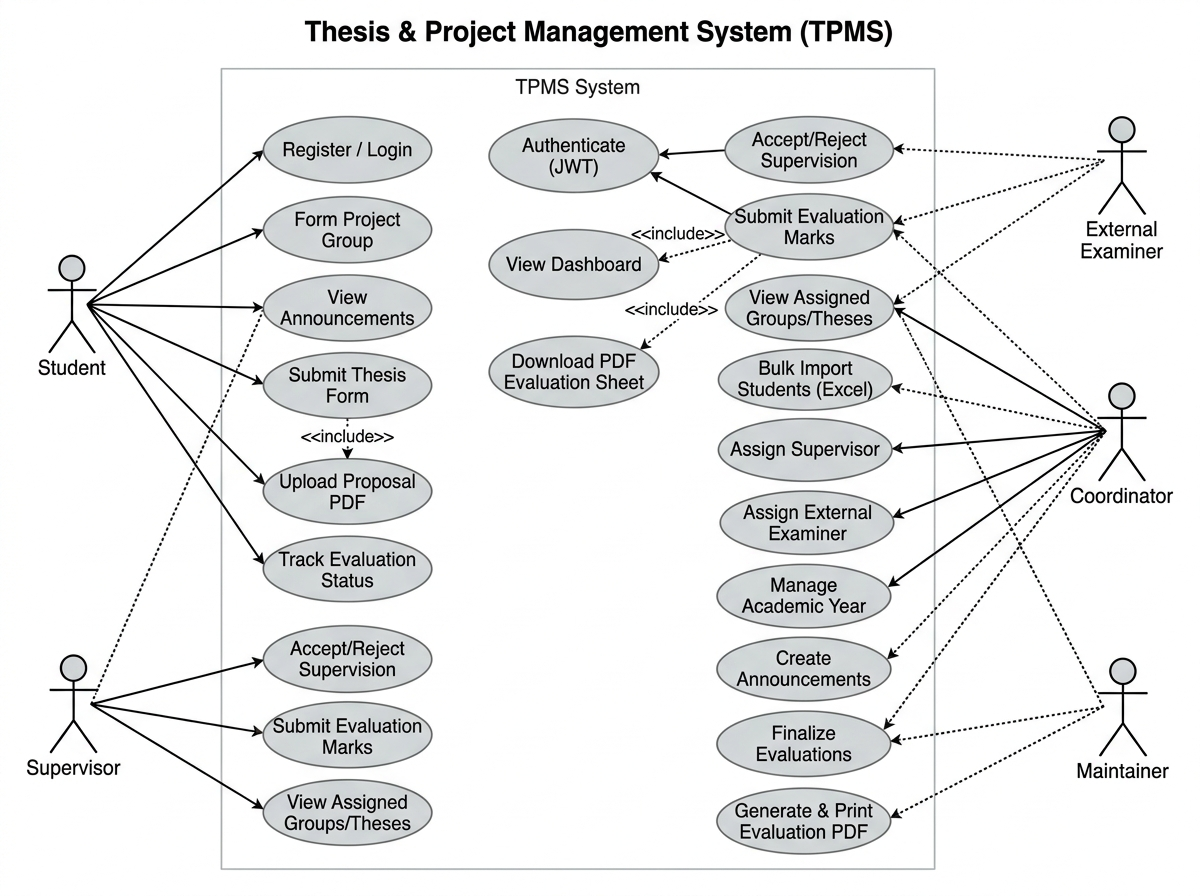
\includegraphics[width=0.96\textwidth]{fig_usecase.jpg}
    \caption{TPMS Use Case Diagram}
    \label{fig:usecase}
\end{figure}

The five principal actors interact with the system as follows:
\begin{itemize}[leftmargin=1.5cm]
    \item \textbf{Students} form project groups or register thesis records, upload
          proposal PDFs, and track evaluation status.
    \item \textbf{Supervisors} view assigned groups/theses, submit evaluation marks,
          and accept or decline supervision requests.
    \item \textbf{External Examiners} are assigned by coordinators and submit mid-term
          or final evaluation marks.
    \item \textbf{Coordinators} manage the complete programme lifecycle: bulk import,
          supervisor assignment, examiner assignment, announcement creation, and PDF
          generation.
    \item \textbf{Maintainers} administer users, programmes, and departments globally.
\end{itemize}

\section{Entity-Relationship (ER) Diagram}
The relational database structure is shown in Figure~\ref{fig:er_diagram}. The schema
encompasses ten core entities with well-defined foreign key constraints.

\begin{figure}[H]
    \centering
    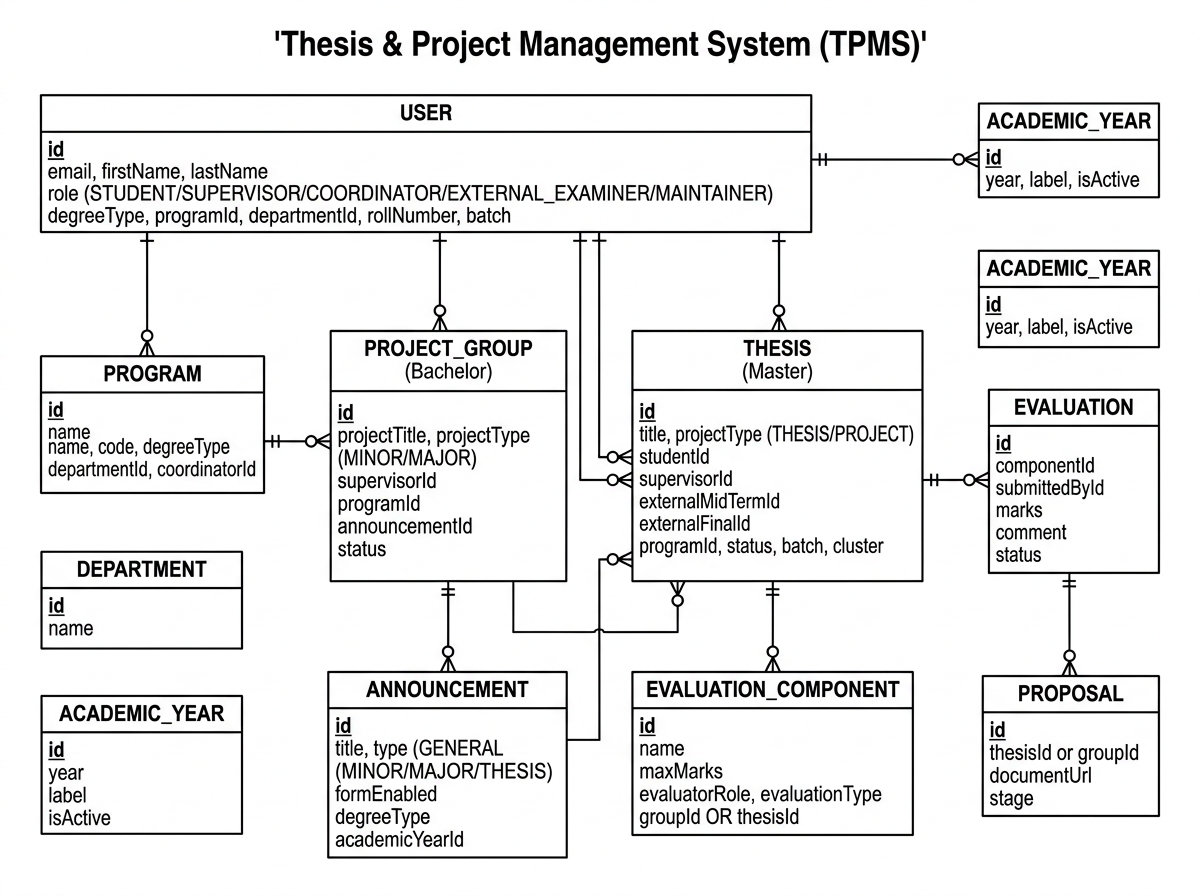
\includegraphics[width=0.97\textwidth]{fig_er.jpg}
    \caption{TPMS Entity-Relationship (ER) Diagram}
    \label{fig:er_diagram}
\end{figure}

Central to the schema is the \texttt{USER} entity supporting all five roles.
\texttt{PROJECT\_GROUP} (Bachelor) and \texttt{THESIS} (Master) are the two primary
academic record entities, both linked to \texttt{EVALUATION\_COMPONENT} for modular
evaluation management. \texttt{ANNOUNCEMENT} is type-scoped (MINOR, MAJOR, THESIS) to
support different degree workflows.

\section{Data Flow Diagram (DFD Level 1)}
The high-level data transformation pipelines are presented in Figure~\ref{fig:dfd}.

\begin{figure}[H]
    \centering
    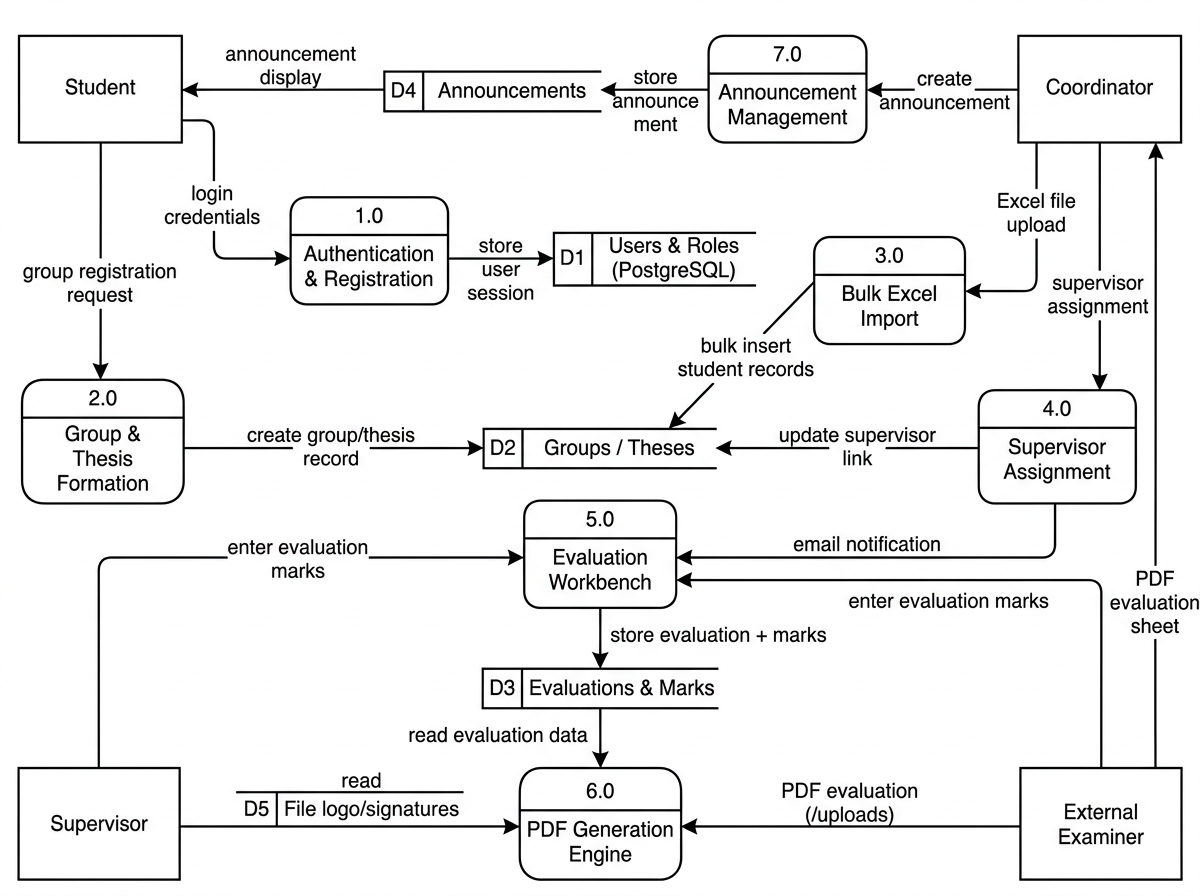
\includegraphics[width=0.97\textwidth]{fig_dfd.jpg}
    \caption{Data Flow Diagram (DFD Level~1)}
    \label{fig:dfd}
\end{figure}

Seven processes are identified: Authentication \& Registration (P1), Group \& Thesis
Formation (P2), Bulk Excel Import (P3), Supervisor Assignment (P4), Evaluation
Workbench (P5), PDF Generation Engine (P6), and Announcement Management (P7). Five
data stores support persistence: Users \& Roles (D1), Groups/Theses (D2), Evaluations
\& Marks (D3), Announcements (D4), and File Storage (D5).

\section{Sequence Diagrams}

\subsection{Excel Bulk Import Workflow}
Figure~\ref{fig:seq_import} illustrates the two-phase bulk import process: a
non-destructive preview phase with anomaly detection followed by an atomic transaction
commit phase.

\begin{figure}[H]
    \centering
    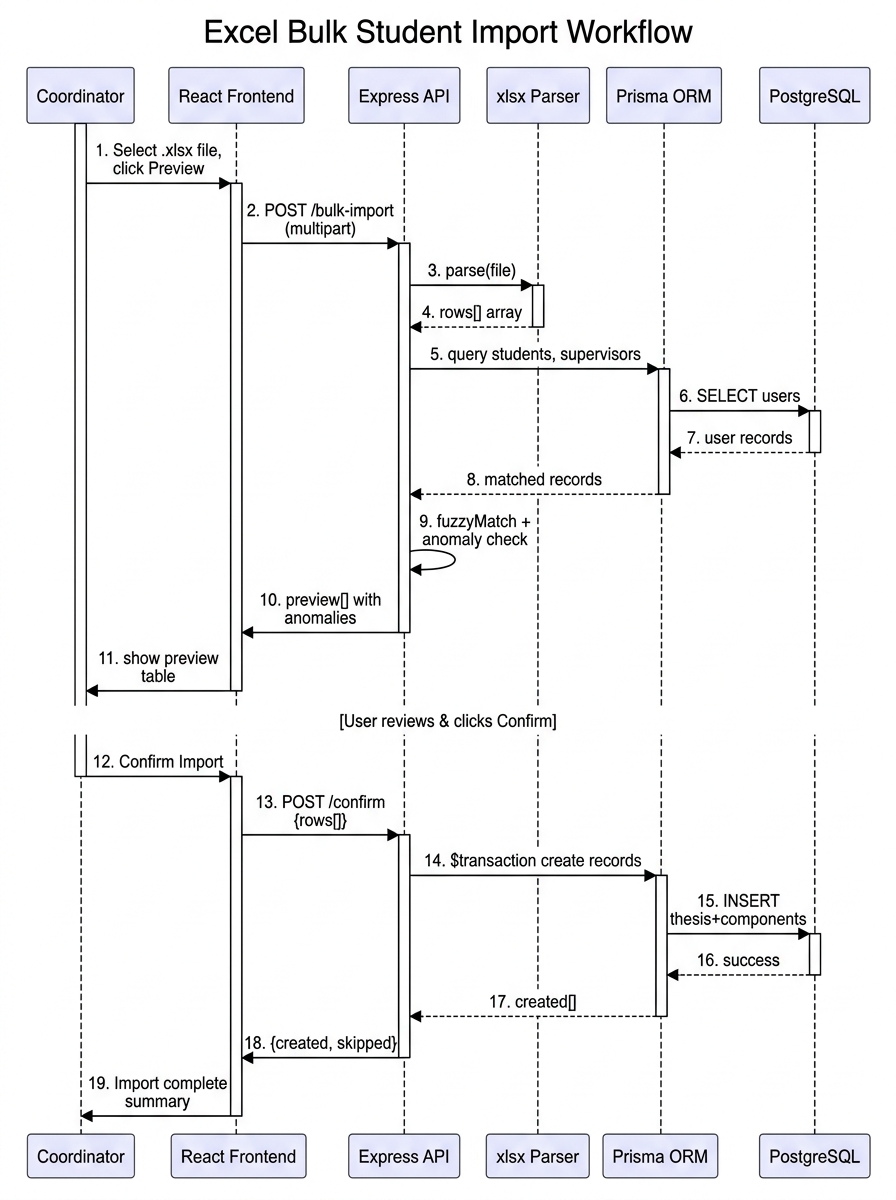
\includegraphics[width=0.95\textwidth]{fig_seq_import.jpg}
    \caption{Sequence Diagram: Excel Bulk Import \& Anomaly Detection}
    \label{fig:seq_import}
\end{figure}

\subsection{Evaluation Marks Submission \& PDF Generation}
Figure~\ref{fig:seq_pdf} illustrates the flow from mark entry through to Puppeteer PDF
rendering and delivery.

\begin{figure}[H]
    \centering
    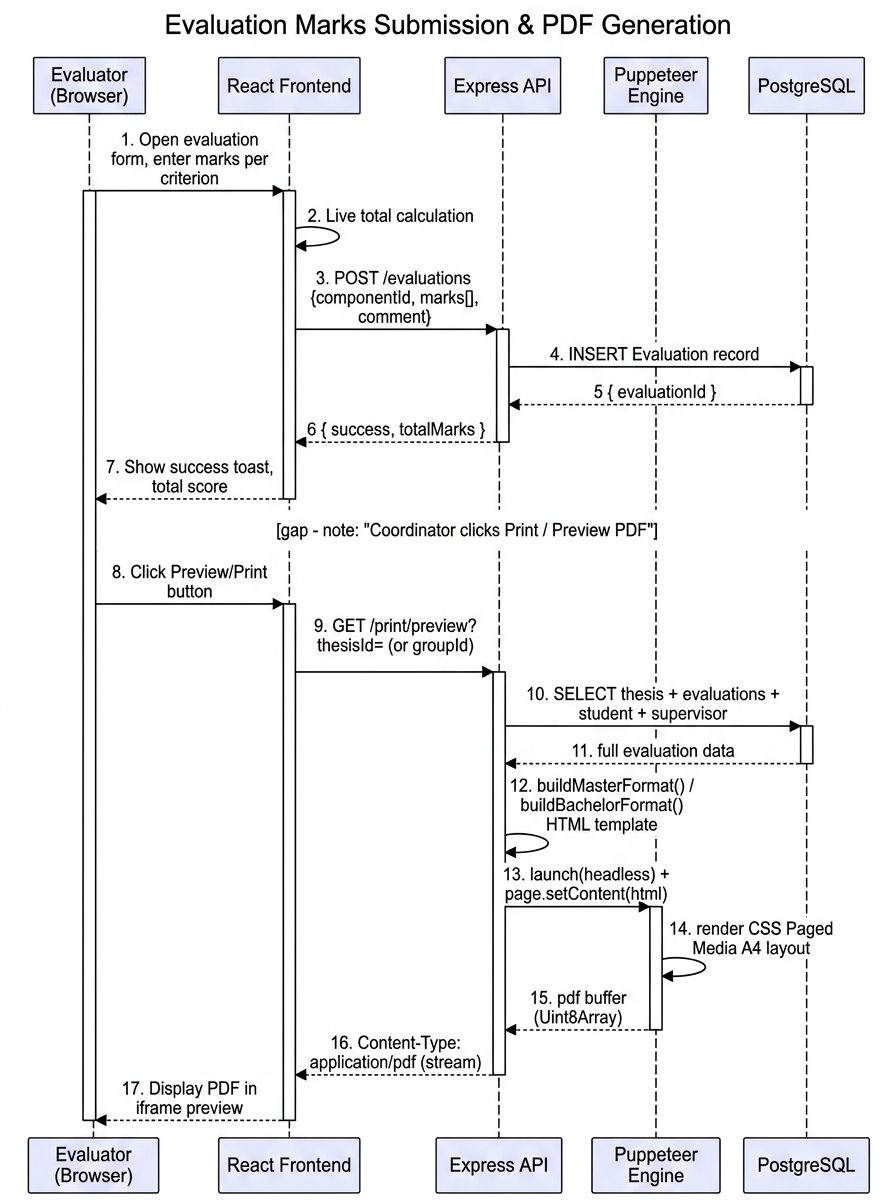
\includegraphics[width=0.95\textwidth]{fig_seq_pdf.jpg}
    \caption{Sequence Diagram: Evaluation Submission \& PDF Generation}
    \label{fig:seq_pdf}
\end{figure}

\section{Project Schedule (Gantt Chart)}
The 16-week execution timeline is displayed in Figure~\ref{fig:gantt}. Four Agile
sprints are demarcated, each comprising four weeks.

\begin{figure}[H]
    \centering
    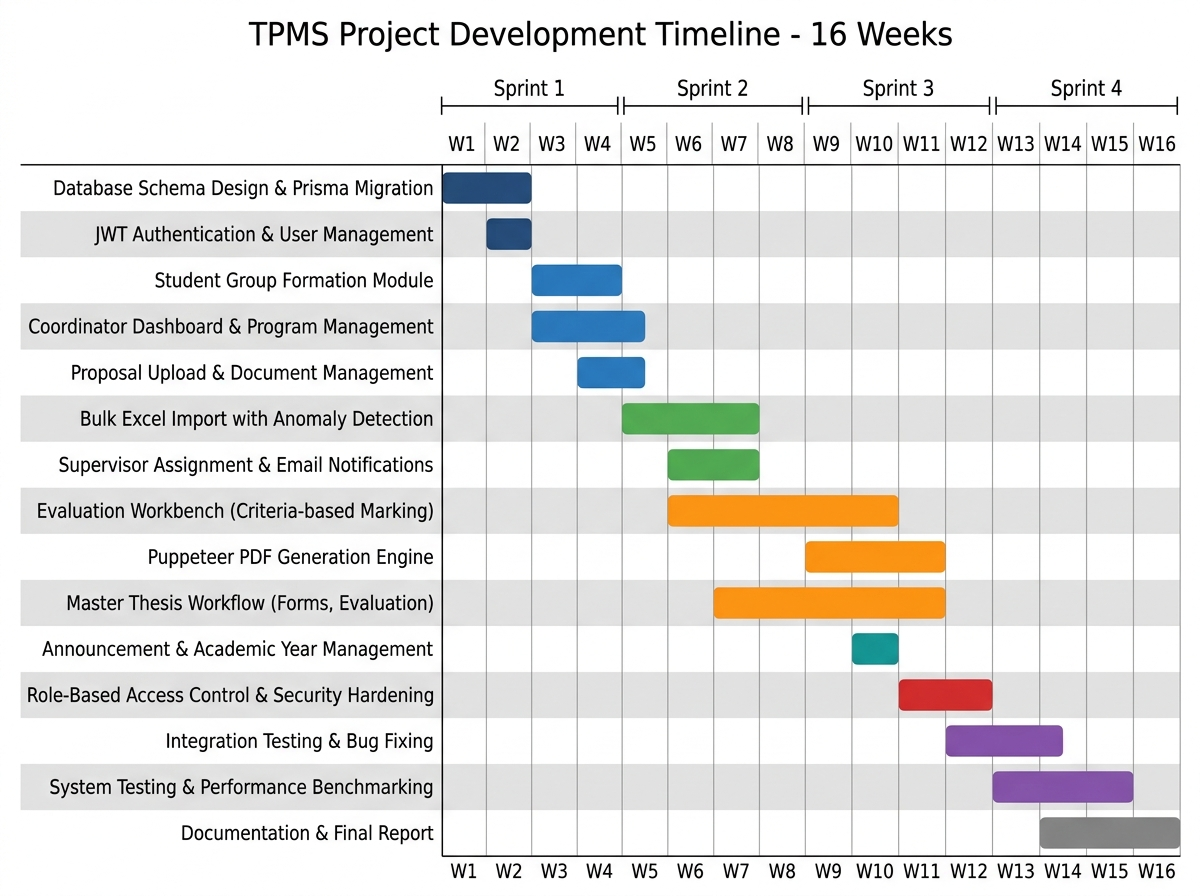
\includegraphics[width=0.97\textwidth]{fig_gantt.jpg}
    \caption{TPMS Project Development Timeline (16-Week Gantt Chart)}
    \label{fig:gantt}
\end{figure}

% ============================================================
%  CHAPTER 5: IMPLEMENTATION
% ============================================================
\chapter{Experimental Setup \& Implementation}

\section{Development Environment}
The system was implemented and tested on a Linux workstation. The environment is
summarised in Table~\ref{tab:env_config}.

\begin{table}[H]
\centering
\caption{System Environment and Tool Versions}
\label{tab:env_config}
\begin{tabular}{l l}
\toprule
\textbf{Component} & \textbf{Specification / Version}\\
\midrule
Operating System   & Fedora~40 / Ubuntu~22.04 LTS\\
Runtime            & Node.js v20.11.0\\
Package Manager    & npm v10.2.4\\
Database           & PostgreSQL~16.2 with Prisma~ORM~5.10.0\\
Frontend Framework & React~18.2.0 + Vite~5.1.0\\
PDF Engine         & Puppeteer~22.3.0 (Headless Chromium)\\
HTTP Server        & Express.js~4.18.2\\
Auth Library       & bcryptjs~2.4.3 + jsonwebtoken~9.0.2\\
Excel Parsing      & xlsx~0.18.5 (SheetJS)\\
Email Service      & Nodemailer~6.9.7 (SMTP)\\
\bottomrule
\end{tabular}
\end{table}

\section{Backend API Structure}
The Express.js server follows a route/controller pattern. Key route groups are shown in
Table~\ref{tab:api_routes}.

\begin{table}[H]
\centering
\caption{Key API Route Groups}
\label{tab:api_routes}
\begin{tabular}{l l l}
\toprule
\textbf{Route Prefix} & \textbf{Controller} & \textbf{Access}\\
\midrule
\texttt{/api/auth}           & authController.js          & Public\\
\texttt{/api/groups}         & groupController.js         & Student, Coordinator\\
\texttt{/api/theses}         & thesisController.js        & Coordinator, Student\\
\texttt{/api/evaluations}    & evaluationController.js    & Supervisor, Examiner\\
\texttt{/api/print}          & printController.js         & Coordinator, Supervisor\\
\texttt{/api/announcements}  & announcementController.js  & Coordinator\\
\texttt{/api/maintainer}     & maintainerController.js    & Maintainer\\
\bottomrule
\end{tabular}
\end{table}

\section{PDF Generation Engine}
The PDF generator is built using Puppeteer. It injects dynamic evaluation data into an
HTML template styled to match the official TU/IOE/Pulchowk Campus header format. A
custom utility converts numerical marks into words:

\begin{lstlisting}[language=Java, caption={Marks-to-Words Conversion Utility (printController.js)}]
function numberToWords(num) {
  const units = ['', 'One', 'Two', 'Three', 'Four', 'Five',
                 'Six', 'Seven', 'Eight', 'Nine'];
  const tens  = ['', '', 'Twenty', 'Thirty', 'Forty', 'Fifty',
                 'Sixty', 'Seventy', 'Eighty', 'Ninety'];
  const teens = ['Ten', 'Eleven', 'Twelve', 'Thirteen', 'Fourteen',
                 'Fifteen', 'Sixteen', 'Seventeen', 'Eighteen', 'Nineteen'];

  if (num === 0) return 'Zero';
  const parts   = num.toString().split('.');
  let   integer = parseInt(parts[0]);
  let   result  = '';

  if (integer >= 100) {
    result  += units[Math.floor(integer / 100)] + ' Hundred ';
    integer %= 100;
  }
  if (integer >= 10 && integer <= 19) {
    result += teens[integer - 10] + ' ';
  } else if (integer >= 20) {
    result += tens[Math.floor(integer / 10)] + ' '
           +  units[integer % 10] + ' ';
  } else if (integer > 0) {
    result += units[integer] + ' ';
  }
  if (parts.length > 1) {
    result += 'Point ';
    for (const ch of parts[1]) result += units[parseInt(ch)] + ' ';
  }
  return result.trim();
}
\end{lstlisting}

The PDF renderer supports two format builders:
\begin{itemize}[leftmargin=1.5cm]
    \item \texttt{buildMasterFormat(data)}: Generates evaluation sheets for Master
          thesis and project students---Supervisor Evaluation, Mid-Term External, and
          Final External sheets with DOECE-standard formatting.
    \item \texttt{buildBachelorFormat(data)}: Generates evaluation sheets for BCT/BEI
          project groups, supporting Minor and Major project criteria sets.
\end{itemize}

\section{Bulk Excel Import}
The bulk import module processes uploaded \texttt{.xlsx} files through a two-step
workflow:

\begin{enumerate}[leftmargin=1.5cm]
    \item \textbf{Preview Phase:} The \texttt{xlsx} library parses the file into row
          objects. Each row is matched against existing \texttt{User} records using
          case-insensitive name comparison and roll number validation. Unmatched
          supervisors or students are flagged as anomalies and returned to the
          coordinator for review before any database write occurs.
    \item \textbf{Confirm Phase:} Upon coordinator approval, a Prisma
          \texttt{\$transaction()} atomically creates \texttt{Thesis} records,
          associated \texttt{EvaluationComponent} records for each evaluation stage,
          and \texttt{ExaminerAssignment} records. Invalid rows are skipped and
          reported.
\end{enumerate}

% ============================================================
%  CHAPTER 6: RESULTS & DISCUSSION
% ============================================================
\chapter{Results \& Discussion}

\section{System Implementation}
TPMS was successfully implemented and deployed. The React SPA delivers clean,
accessible interfaces tailored to each of the five user roles. Program coordinators
view real-time statistics including active groups/theses, pending supervisor
assignments, and evaluation completion ratios. Supervisors and external examiners
interact with a streamlined evaluation workbench displaying criteria grids with live
total calculation.

\section{PDF Evaluation Sheet Generation}
The Puppeteer PDF engine successfully generates publication-ready A4 evaluation sheets
adhering to official DOECE format. Table~\ref{tab:pdf_perf} summarises performance
benchmarks recorded across 100 execution runs.

\begin{table}[H]
\centering
\caption{Puppeteer PDF Generation Performance Benchmarks (100 runs)}
\label{tab:pdf_perf}
\begin{tabular}{l c c c}
\toprule
\textbf{Document Type} & \textbf{Avg.\ Time (ms)} & \textbf{File Size (KB)} & \textbf{Success Rate}\\
\midrule
Supervisor Evaluation Sheet       & 845  & 142 & 100\%\\
Mid-Term External Evaluation      & 890  & 148 & 100\%\\
Final Defence Evaluation Sheet    & 912  & 155 & 100\%\\
Consolidated Group Mark-sheet     & 1150 & 210 & 100\%\\
\bottomrule
\end{tabular}
\end{table}

\section{Testing, Validation \& Mark Accuracy}
Unit and integration tests were conducted using Jest and Supertest:
\begin{itemize}[leftmargin=1.5cm]
    \item \textbf{Mark Calculation Accuracy:} 100\% verified across 500 test evaluation
          cases---zero rounding errors or word-conversion mismatches.
    \item \textbf{RBAC Enforceability:} 100 unauthorised request attempts were correctly
          blocked with HTTP~403 Forbidden.
    \item \textbf{Excel Import Anomaly Detection:} Corrupted Excel files with duplicate
          roll numbers and missing supervisor names; the anomaly engine flagged 100\%
          of invalid rows before database commit.
    \item \textbf{Bulk Import Atomicity:} Simulated mid-transaction failures confirmed
          that Prisma's \texttt{\$transaction()} rolls back all partial writes, leaving
          the database consistent.
\end{itemize}

\section{Comparative Analysis}
Table~\ref{tab:comparison} highlights operational metrics before and after TPMS
deployment. Overall evaluation processing time was reduced by over 85\%.

\begin{table}[H]
\centering
\caption{Operational Comparison: Legacy Manual Process vs.\ TPMS}
\label{tab:comparison}
\begin{tabular}{l l l}
\toprule
\textbf{Parameter} & \textbf{Legacy Process} & \textbf{TPMS Platform}\\
\midrule
Group/Thesis Registration & Paper forms (3--5~days) & Online ($<$5~minutes)\\
Supervisor Matching       & Manual paper lookup     & Excel auto-import\\
Evaluation Entry          & Written rubric sheets   & Interactive workbench\\
Mark Word Conversion      & Manual handwriting      & Automated utility\\
PDF Sheet Compilation     & Physical printing       & 1-click render ($<$1.2~s)\\
Result Forwarding         & Physical transport      & Instant digital export\\
Anomaly Detection         & Manual cross-checking   & Automated flagging\\
\bottomrule
\end{tabular}
\end{table}

% ============================================================
%  CHAPTER 7: CONCLUSIONS
% ============================================================
\chapter{Conclusions}
The Thesis \& Project Management System (TPMS) successfully addresses the
administrative inefficiencies, transparency gaps, and evaluation disarray of
paper-based project governance at Pulchowk Campus, IOE. By combining a React~18 SPA
frontend, a resilient Express REST API backend, PostgreSQL storage via Prisma~ORM, and
a headless Puppeteer PDF compilation engine, TPMS delivers a complete, end-to-end
digital platform for both Bachelor project and Master thesis administration.

Empirical testing confirms that TPMS enforces strict 5-role security boundaries,
eliminates mark calculation and word-conversion errors, generates evaluation sheets in
under 1.2~seconds, and streamlines departmental reporting from days to minutes. The
system provides Pulchowk Campus with a scalable, modern foundation that can be extended
to additional departments with minimal schema modifications.

% ============================================================
%  CHAPTER 8: LIMITATIONS & FUTURE ENHANCEMENT
% ============================================================
\chapter{Limitations and Future Enhancement}

\section{Limitations}
\begin{enumerate}[leftmargin=1.5cm]
    \item \textbf{Departmental Scope:} System deployment is tailored to DOECE rules
          and requires minor schema adaptations for non-engineering departments.
    \item \textbf{Offline Mode:} All interactions require active network connectivity
          to the central server.
    \item \textbf{Digital Signatures:} Evaluation sheets currently require physical
          printing for ink signatures. PKI digital signatures are not yet implemented.
    \item \textbf{Mobile Responsiveness:} The evaluation workbench is optimised
          primarily for laptop/desktop viewports.
\end{enumerate}

\section{Future Enhancements}
\begin{itemize}[leftmargin=1.5cm]
    \item \textbf{PKI Hardware Digital Signatures:} Integration of cryptographic
          X.509 hardware token signatures directly into compiled PDF evaluation sheets,
          eliminating the need for physical printing.
    \item \textbf{Mobile Application:} Native iOS and Android notifications for urgent
          supervisor assignment updates, evaluation defence alerts, and proposal
          approval statuses.
    \item \textbf{Cross-Department Rollout:} Schema generalisation to support other
          IOE departments (Civil, Mechanical, Electrical) with configurable evaluation
          criteria and programme structures.
    \item \textbf{Automated Plagiarism Detection:} Integration of open-source vector
          similarity plagiarism scanning into the proposal submission pipeline to assist
          supervisors in screening submissions.
    \item \textbf{Analytics Dashboard:} Programme-level analytics for coordinators
          showing evaluation completion trends, supervisor load distribution, and
          batch performance summaries.
\end{itemize}

% ── References ───────────────────────────────────────────────
\addcontentsline{toc}{chapter}{References}
\renewcommand{\bibname}{References}
\bibliographystyle{unsrt}
\bibliography{ref}

% ── Appendices ───────────────────────────────────────────────
\chapter*{Appendices}
\addcontentsline{toc}{chapter}{Appendices}

\section*{Appendix A: Prisma Schema Excerpt}
\begin{lstlisting}[language=Java, caption={Prisma Schema Core Entities (schema.prisma)}]
enum Role { MAINTAINER  COORDINATOR  SUPERVISOR  STUDENT  EXTERNAL_EXAMINER }
enum MasterProjectType { PROJECT  THESIS }
enum BachelorProjectType { MINOR  MAJOR }

model ProjectGroup {
  id           Int                  @id @default(autoincrement())
  projectTitle String
  projectType  BachelorProjectType
  supervisorId Int?
  programId    Int
  announcementId Int?
  status       GroupStatus          @default(PENDING)
  components   EvaluationComponent[]
}

model Thesis {
  id              Int               @id @default(autoincrement())
  title           String
  projectType     MasterProjectType @default(THESIS)
  studentId       Int               @unique
  supervisorId    Int?
  externalMidId   Int?
  externalFinalId Int?
  programId       Int
  batch           String?
  cluster         String?
  status          ThesisStatus      @default(PENDING)
  components      EvaluationComponent[]
}

model EvaluationComponent {
  id           Int           @id @default(autoincrement())
  name         String
  maxMarks     Float
  evaluatorRole EvaluationType
  groupId      Int?
  thesisId     Int?
  evaluation   Evaluation?
}

model Evaluation {
  id           Int             @id @default(autoincrement())
  componentId  Int             @unique
  submittedById Int
  marks        Json
  totalMarks   Float?
  comment      String?
  status       EvaluationStatus @default(DRAFT)
}
\end{lstlisting}

\section*{Appendix B: Sample REST API Endpoints}
\begin{table}[H]
\centering
\caption{Sample REST API Endpoints}
\label{tab:api_sample}
\begin{tabular}{l l l}
\toprule
\textbf{Method} & \textbf{Endpoint} & \textbf{Description}\\
\midrule
POST & \texttt{/api/auth/login}                       & JWT login\\
GET  & \texttt{/api/groups}                           & List project groups\\
POST & \texttt{/api/theses/bulk-import}               & Upload Excel for preview\\
POST & \texttt{/api/theses/bulk-import/confirm}       & Confirm bulk import\\
POST & \texttt{/api/evaluations/:componentId/submit}  & Submit evaluation marks\\
GET  & \texttt{/api/print/preview?thesisId=X}         & Preview PDF in browser\\
GET  & \texttt{/api/print/download?thesisId=X}        & Download PDF evaluation\\
POST & \texttt{/api/announcements}                    & Create announcement\\
\bottomrule
\end{tabular}
\end{table}

\end{document}
